\documentclass[aspectratio=169]{beamer}

% --- lualatex preamble ------------------------------------------------------
% Unlike pdflatex, no \usepackage[utf8]{inputenc} and no \usepackage[T1]{fontenc}.
% lualatex is Unicode-native and uses OpenType system fonts directly.
\usepackage{fontspec}
\usepackage{unicode-math}

% --- theme -----------------------------------------------------------------
\usetheme{metropolis}
\usepackage{appendixnumberbeamer}

% --- fonts (Fira is the metropolis house style; swap freely) ---------------
\setsansfont{Fira Sans}
\setmonofont{Fira Mono}
\setmathfont{Fira Math}        % shipped by texlive-fontsextra

% --- packages --------------------------------------------------------------
\usepackage{tikz}
\usetikzlibrary{positioning, arrows.meta, calc, fit, backgrounds, shapes.geometric}

% --- colors for the mapgen-workflow figure ---------------------------------
\definecolor{cInput}{HTML}{E8F0FE}
\definecolor{cPerc}{HTML}{FDE9D9}
\definecolor{cLift}{HTML}{E2F0D9}
\definecolor{cGeo}{HTML}{FFF2CC}
\definecolor{cAsm}{HTML}{F4CCCC}
\definecolor{cResult}{HTML}{D9D2E9}
\definecolor{cGen}{HTML}{ECECEC}
\definecolor{cNo}{HTML}{C0504D}   % muted red accent matching the pastel palett, for positive accentuatione
\definecolor{cYes}{HTML}{6AA84F}   % muted green accent matching the pastel palette, for positive accentuation
\usepackage{pgfplots}
\pgfplotsset{compat=1.18}      % match the installed version
\usepackage{minted}            % needs --shell-escape (set in latexmkrc)
\usepackage{booktabs}
\usepackage{hyperref}

% --- metadata --------------------------------------------------------------
\title{Map Localization for ADAS}
%\subtitle{A subtitle that says more}
\author{Michael Schweitzer}
\date{\today}

\begin{document}

\maketitle

\begin{frame}{Outline}
  \tableofcontents
\end{frame}

% ---------------------------------------------------------------------------
\section{Motivation}

\begin{frame}{Why we care}
  \begin{itemize}
    \item One reason
    \item Another reason
    \item A third one with \alert{emphasis}
  \end{itemize}
\end{frame}

% ---------------------------------------------------------------------------
\section{A diagram}

\begin{frame}{TikZ works exactly like under pdflatex}
  \centering
  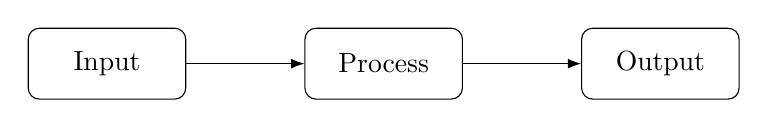
\begin{tikzpicture}[
      node distance=15mm,
      every node/.style={draw, rounded corners, minimum height=9mm, minimum width=20mm}
    ]
    \node (a) {Input};
    \node[right=of a] (b) {Process};
    \node[right=of b] (c) {Output};
    \draw[-Latex] (a) -- (b);
    \draw[-Latex] (b) -- (c);
  \end{tikzpicture}
\end{frame}

% ---------------------------------------------------------------------------
\section{A plot}

\begin{frame}{Benchmark: runtime vs.\ input size}
  \centering
  \begin{tikzpicture}
    \begin{axis}[
        width=0.85\textwidth, height=0.65\textheight,
        xlabel={Input size $n$}, ylabel={Runtime (ms)},
        xmode=log, ymode=log,
        log basis x=10, log basis y=10,
        grid=both, major grid style={black!15}, minor grid style={black!5},
        legend pos=north west,
        legend cell align=left,
        thick,
    ]
      % naive: O(n^2)
      \addplot+[mark=*] coordinates {
        (10, 0.1) (100, 8) (1000, 750) (10000, 72000)
      };
      \addlegendentry{naive $\mathcal{O}(n^2)$}

      % optimized: O(n log n)
      \addplot+[mark=square*] coordinates {
        (10, 0.3) (100, 4) (1000, 55) (10000, 720)
      };
      \addlegendentry{optimized $\mathcal{O}(n \log n)$}
    \end{axis}
  \end{tikzpicture}
\end{frame}

% ---------------------------------------------------------------------------
\section{Some code}

% Frames containing minted/verbatim must be marked [fragile].
\begin{frame}[fragile]{A syntax-highlighted code block}
  \begin{minted}[fontsize=\small, bgcolor=black!5]{python}
def greet(name: str) -> str:
    return f"hello, {name}"
  \end{minted}
\end{frame}

% ---------------------------------------------------------------------------
\section{A video}

% pdfpc-specific: \href{run:...} autostarts and loops the video in pdfpc.
% Works only in pdfpc; other viewers treat it as a plain link.
\begin{frame}[plain]
  \centerline{%
    \href{run:media/a2_perception_2.mp4?autostart\&loop}
         {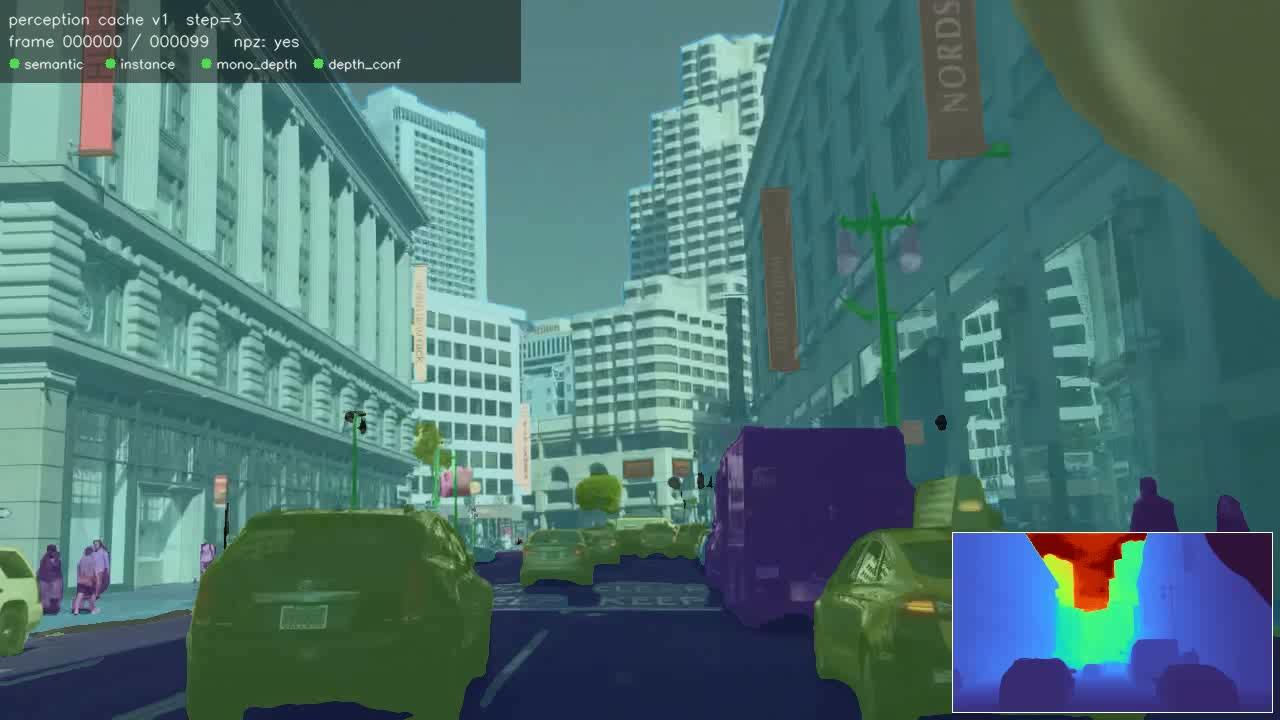
\includegraphics[height=0.95\paperheight]{media/a2_perception_2_poster.jpg}}%
  }
\end{frame}

\begin{frame}[plain]
  \centerline{%
    \href{run:media/a4_tag_kps_class.mp4?autostart\&loop}
         {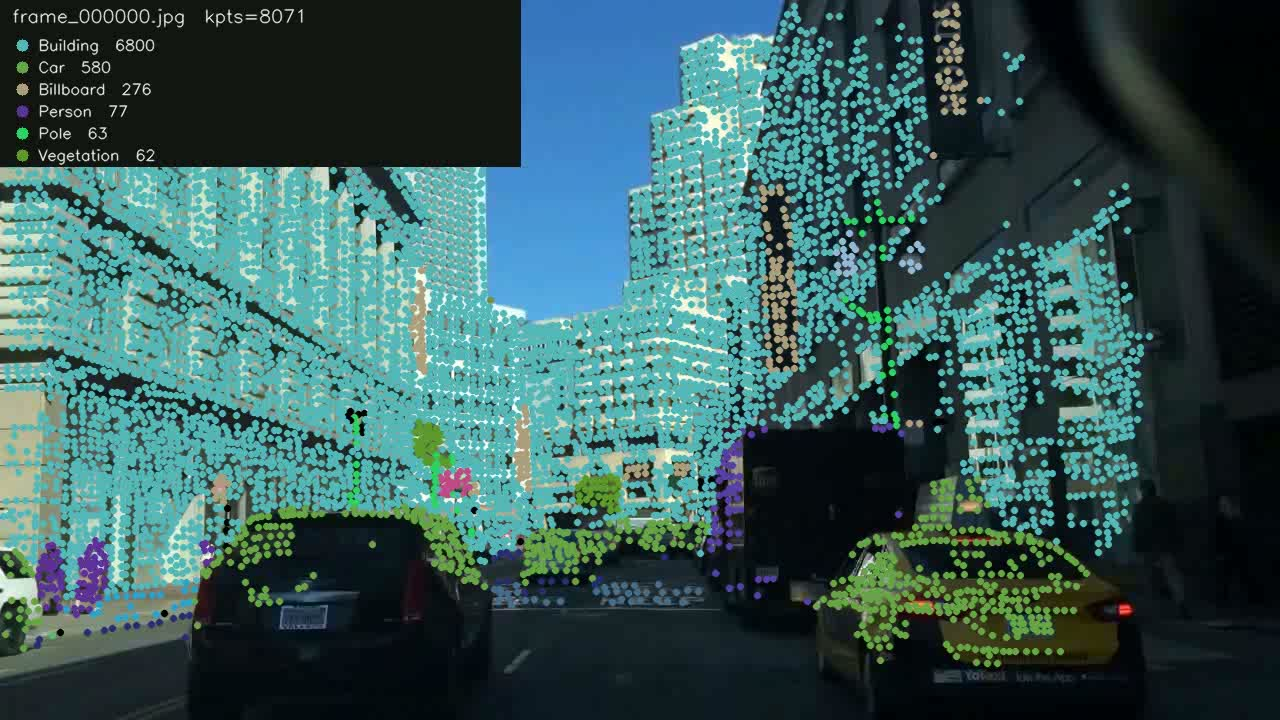
\includegraphics[height=0.95\paperheight]{media/a4_tag_kps_class_poster.jpg}}%
  }
\end{frame}

\begin{frame}[plain]
  \centerline{%
    \href{run:media/a4_tag_kps_depth.mp4?autostart\&loop}
         {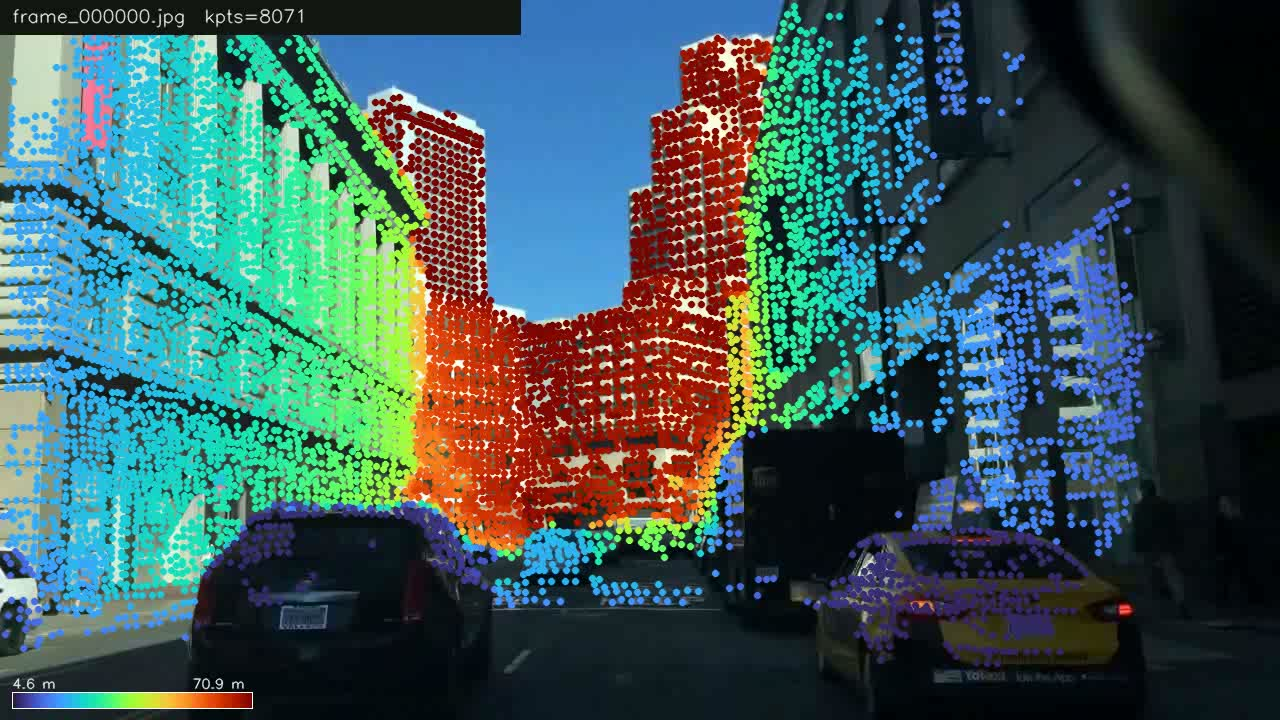
\includegraphics[height=0.95\paperheight]{media/a4_tag_kps_depth_poster.jpg}}%
  }
\end{frame}

\begin{frame}[plain]
  \centerline{%
    \href{run:media/static_dynamic.mp4?autostart\&loop}
         {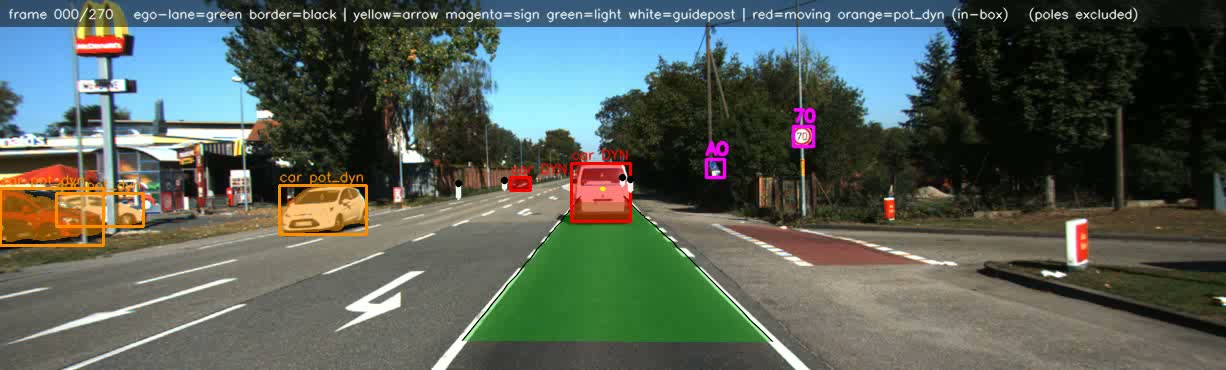
\includegraphics[width=\paperwidth,height=0.95\paperheight,keepaspectratio]{media/static_dynamic_poster.jpg}}%
  }
\end{frame}

\begin{frame}[plain]
  \centerline{%
    \href{run:media/reveal_lift_return.mp4?autostart\&loop}
         {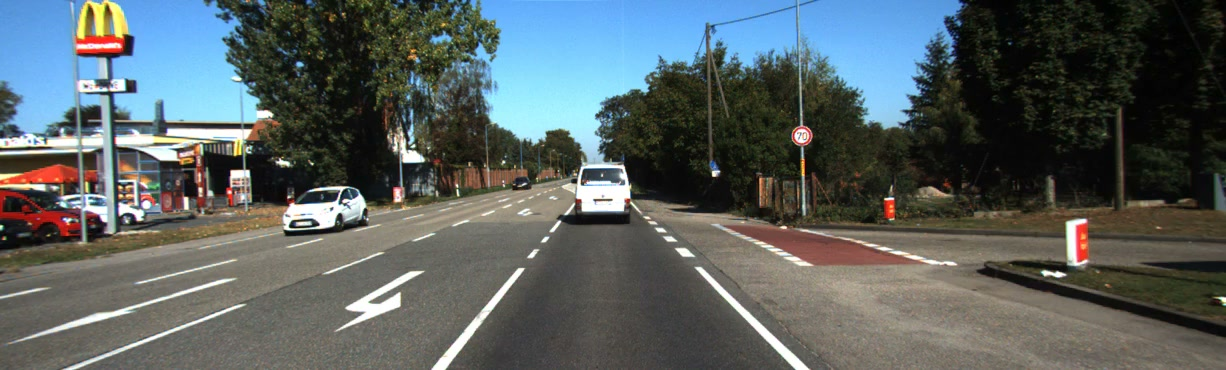
\includegraphics[width=\paperwidth,height=0.95\paperheight,keepaspectratio]{media/reveal_lift_return_poster.jpg}}%
  }
\end{frame}

\begin{frame}[plain]
  % slide rtk_offset
  \begin{tikzpicture}[remember picture, overlay]
    % track-on-satellite image, pushed to the left edge
    \node[anchor=west, inner sep=0] (E)
      at ([xshift=2mm]current page.west)
      {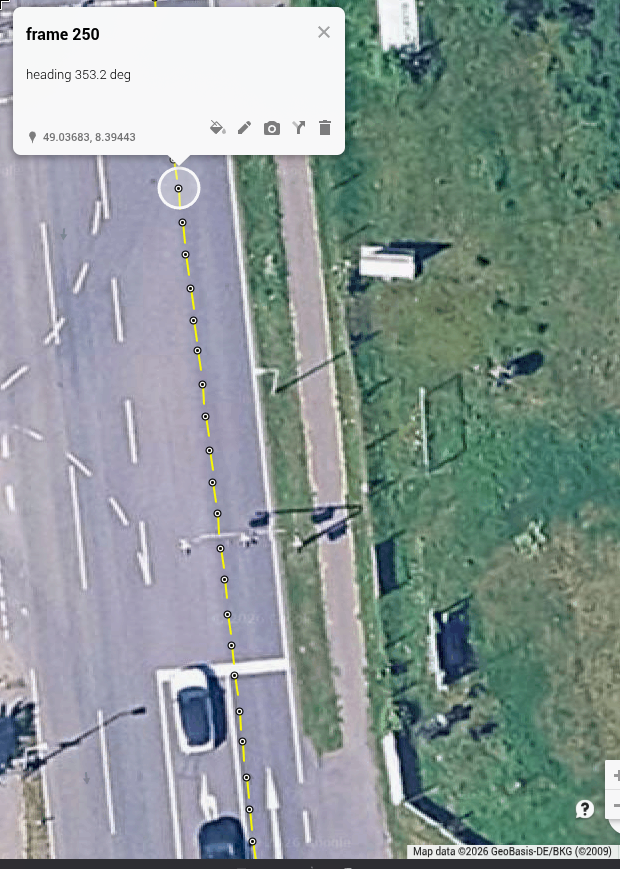
\includegraphics[height=0.92\paperheight]{media/kitti04_track_earth.png}};
    % camera frame of frame 230, bottom-right
    \node[anchor=south east, inner sep=0] (C)
      at ([xshift=-3mm, yshift=3mm]current page.south east)
      {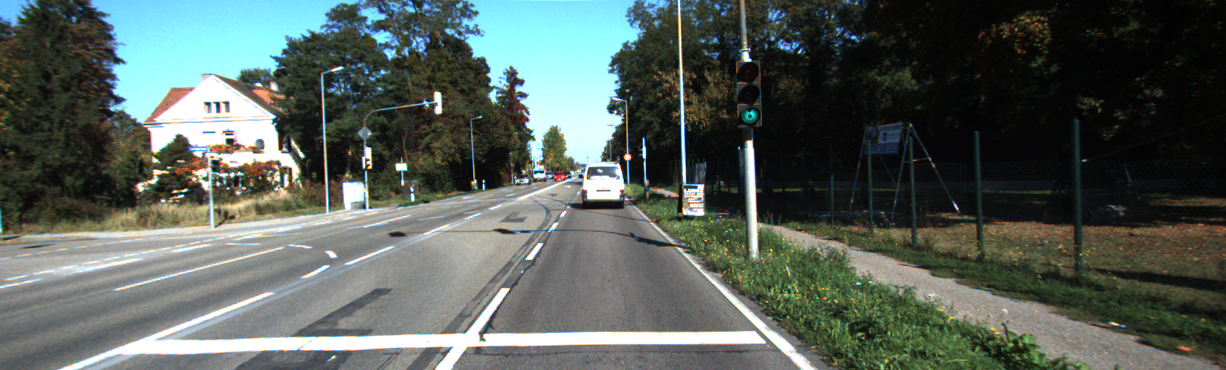
\includegraphics[width=0.52\paperwidth]{media/frame_230_rgb.png}};
    % vertical yellow line through the middle of the frame-230 image
    \draw[yellow, line width=5pt] (C.north) -- (C.south);
    % estimated position of track point 230 inside the earth image.
    % (FX,FY) are fractions of the image box (0,0)=bottom-left .. (1,1)=top-right.
    % Nudge these two numbers if the marker is off the actual point.
    \coordinate (p230) at
      ($($(E.south west)!0.41!(E.south east)$)!0.02!($(E.north west)!0.41!(E.north east)$)$);
    \draw[red, very thick] (p230) circle (2.4mm);
    \node[red, font=\footnotesize\bfseries, anchor=east, xshift=-3mm] at (p230) {230};
    % connector linking the track point to the camera frame
    \draw[-Latex, red, very thick]
      (p230) .. controls +(right:18mm) and +(left:12mm) .. (C.north west);
    % three text-window notes, stacked in the right column above the camera frame
    \node[anchor=north east, inner sep=0] (N1)
      at ([xshift=-5mm, yshift=-5mm]current page.north east)
      {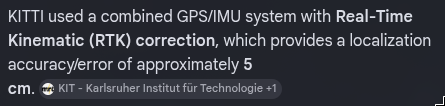
\includegraphics[width=0.40\paperwidth]{media/rtk_offset_note.png}};
    \node[anchor=north east, inner sep=0] (N2)
      at ([yshift=-2mm]N1.south east)
      {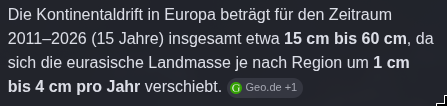
\includegraphics[width=0.40\paperwidth]{media/rtk_drift_note.png}};
    \node[anchor=north east, inner sep=0] (N3)
      at ([yshift=-2mm]N2.south east)
      {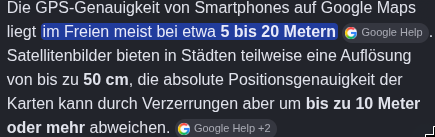
\includegraphics[width=0.40\paperwidth]{media/gps_accuracy_note.png}};
  \end{tikzpicture}
\end{frame}

\begin{frame}[plain]
  \centerline{%
    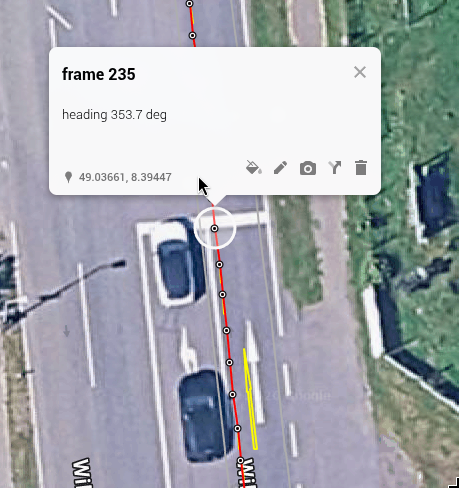
\includegraphics[width=\paperwidth,height=0.95\paperheight,keepaspectratio]{media/kitti04_frame235.png}%
  }
\end{frame}

\begin{frame}[plain]
  \centerline{%
    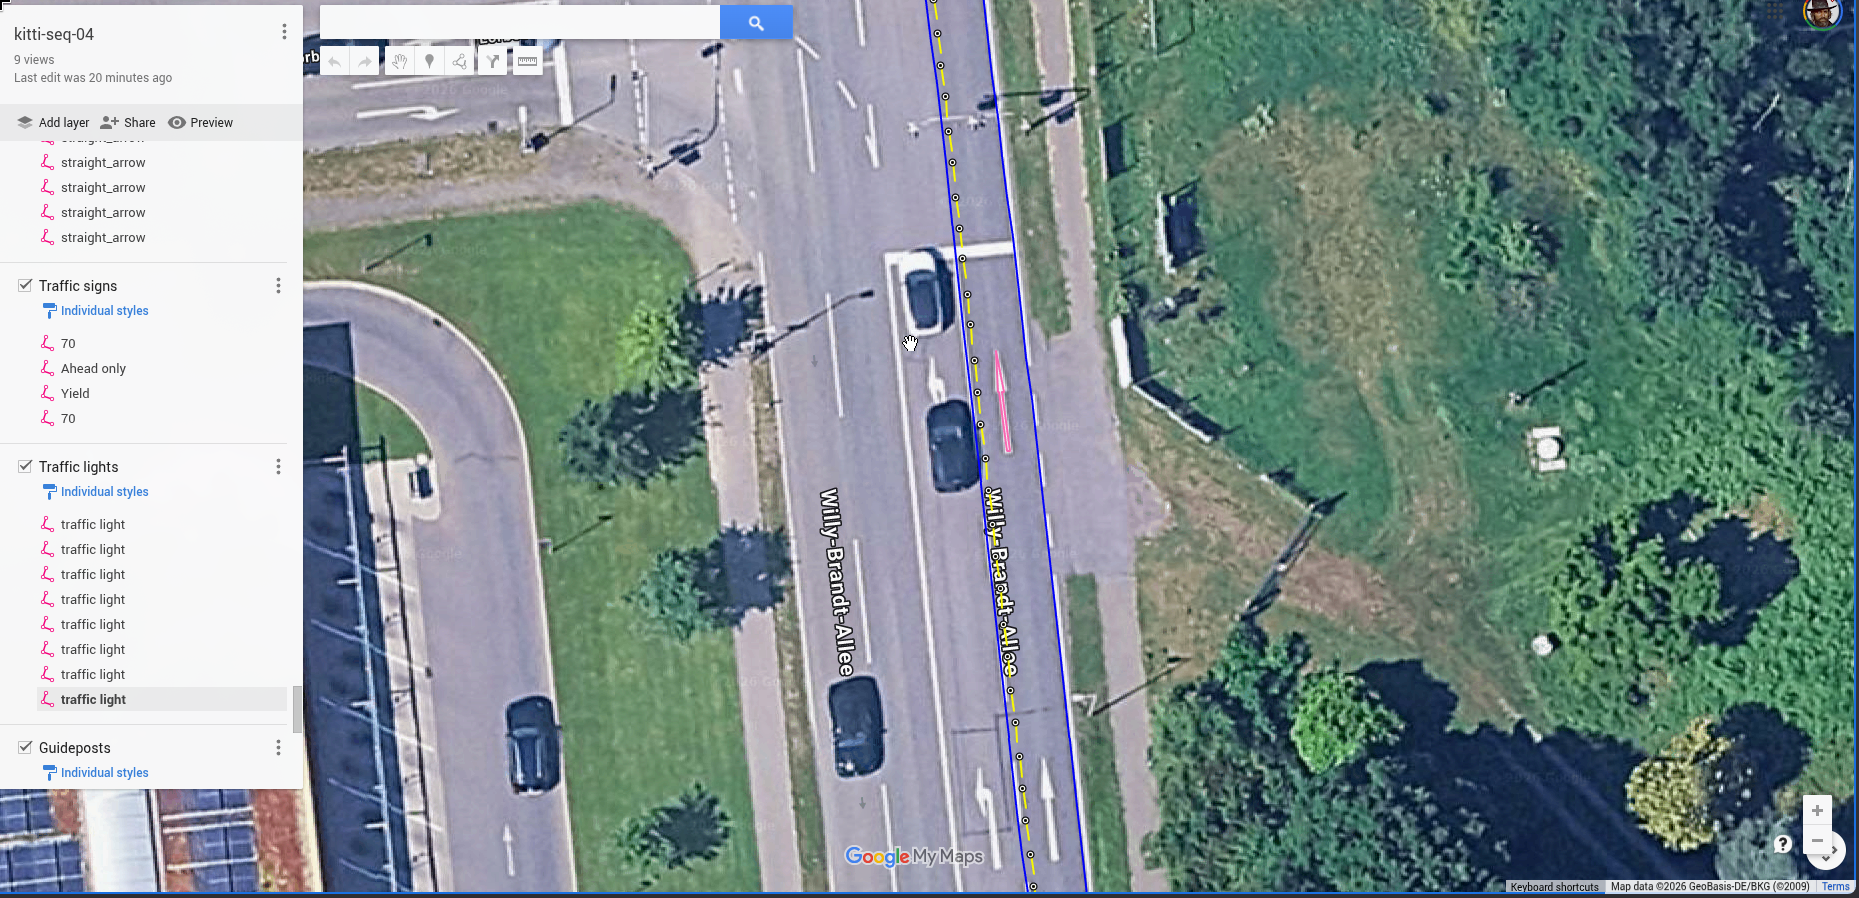
\includegraphics[width=\paperwidth,height=0.95\paperheight,keepaspectratio]{media/kitti04_mymaps_layers.png}%
  }
\end{frame}

% ---------------------------------------------------------------------------
% slide mapgen_workflow — ADAS map-generation pipeline
% (figure body from aivision/docs/mapgen_workflow.tex, scaled to fit the slide)
\begin{frame}{Map Building Workflow} % mapbuild
  \centering
  \vfill
  \resizebox{\textwidth}{!}{%
  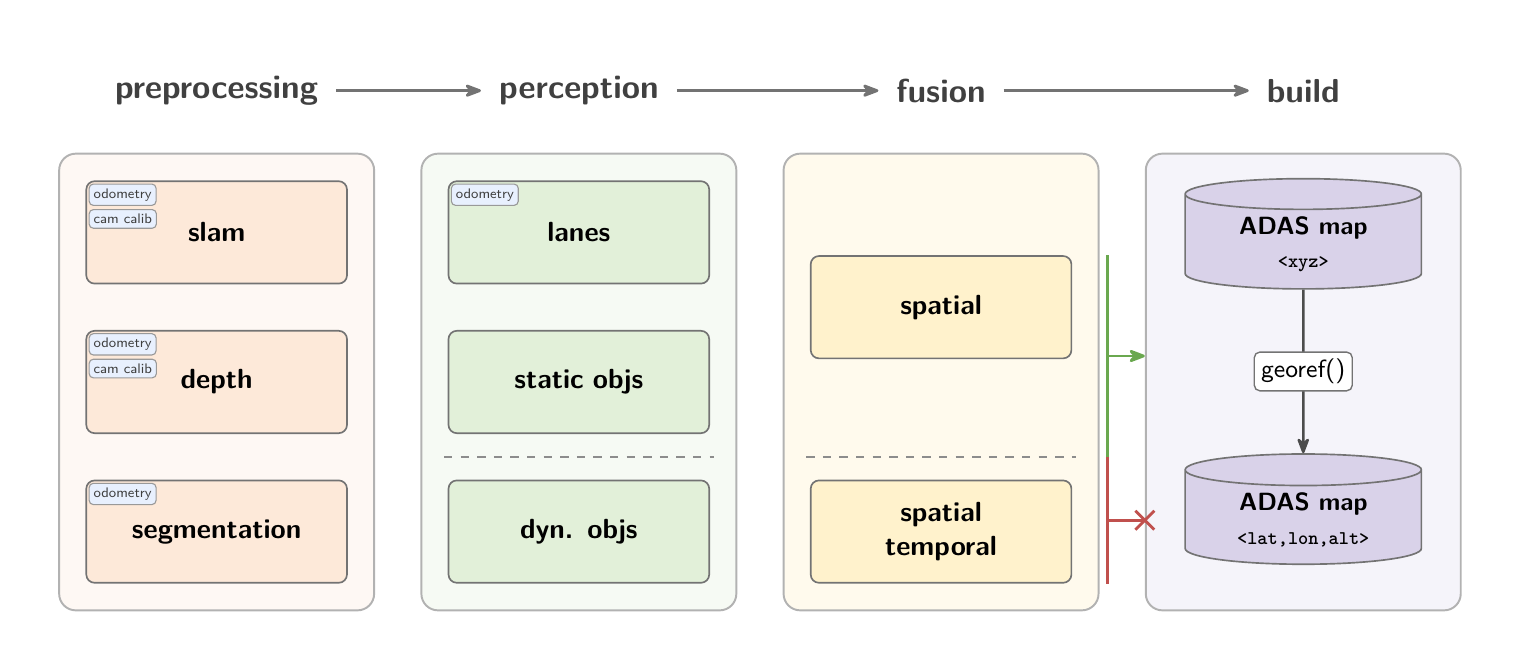
\begin{tikzpicture}[
    font=\sffamily\small,
    >={Stealth[round]},
    % equal column geometry: 4 columns, centers at 0, 4.6, 9.2, 13.8
    box/.style={rounded corners=3pt, draw=black!55, line width=.6pt, align=center,
                text width=31mm, minimum height=13mm, inner sep=3pt, font=\sffamily\bfseries},
    arr/.style={->, line width=.9pt, draw=black!70},
    titlearr/.style={->, line width=1pt, draw=black!55, shorten >=3pt, shorten <=3pt},
    divider/.style={dashed, draw=black!45, line width=.6pt},
    inbadge/.style={fill=cInput, draw=black!40, line width=.4pt, rounded corners=1.5pt,
                    font=\sffamily\tiny, inner sep=1.6pt, anchor=north west, text=black!75},
    groupbox/.style={rounded corners=6pt, draw=black!30, line width=.7pt,
                     minimum width=40mm, minimum height=58mm},
    grouptitle/.style={font=\sffamily\bfseries\large, text=black!75},
    glabel/.style={fill=white, draw=black!55, line width=.5pt, rounded corners=2pt,
                   font=\sffamily\small, inner sep=2.5pt},
    db/.style={cylinder, shape border rotate=90, aspect=0.22, draw=black!55, line width=.6pt,
               fill=cResult, align=center, minimum width=30mm, minimum height=14mm,
               inner sep=2pt, font=\sffamily\bfseries\small},
  ]

  % ---- equal-size column frames (centered at y=-0.9) ----
  \begin{scope}[on background layer]
    \node[groupbox, fill=cPerc!30]   (gpre) at (0,-0.9)    {};
    \node[groupbox, fill=cLift!30]   (gper) at (4.6,-0.9)  {};
    \node[groupbox, fill=cGeo!35]    (gfus) at (9.2,-0.9)  {};
    \node[groupbox, fill=cResult!25] (gcre) at (13.8,-0.9) {};
  \end{scope}

  % ---- preprocessing column (orange) ----
  \node[box, fill=cPerc] (slam)  at (0,1.0)   {slam};
  \node[box, fill=cPerc] (depth) at (0,-0.9)  {depth};
  \node[box, fill=cPerc] (seg)   at (0,-2.8)  {segmentation};

  % ---- perception column (green) ----
  \node[box, fill=cLift] (lanes)    at (4.6,1.0)   {lanes};
  \node[box, fill=cLift] (statobjs)  at (4.6,-0.9)  {static objs};
  \node[box, fill=cLift] (dynobjs) at (4.6,-2.8)  {dyn. objs};

  % ---- fusion column (yellow): two boxes, no input badges ----
  % spatial centered in the upper part (rows 1-2, above the divider); spatial/temporal below it
  \node[box, fill=cGeo] (spatial)  at (9.2,0.05)  {spatial};
  \node[box, fill=cGeo] (spattemp) at (9.2,-2.8)  {spatial\\temporal};

  % ---- create column: ADAS map databases, local (xyz) -> geographic via georef() ----
  \node[db] (db1) at (13.8,0.85)  {ADAS map\\[1pt]{\ttfamily\scriptsize <xyz>}};
  \node[db] (db2) at (13.8,-2.65) {ADAS map\\[1pt]{\ttfamily\scriptsize <lat,lon,alt>}};
  \draw[arr] (db1.south) -- (db2.north) node[midway, glabel] {georef()};

  % ---- input overlays (top-left badges) on preprocessing + perception only ----
  \node[inbadge] (slamin) at ([xshift=.4mm,yshift=-.4mm]slam.north west) {odometry};
  \node[inbadge]          at ([yshift=-.4mm]slamin.south west) {cam calib};
  \node[inbadge] (depin)  at ([xshift=.4mm,yshift=-.4mm]depth.north west) {odometry};
  \node[inbadge]          at ([yshift=-.4mm]depin.south west) {cam calib};
  \node[inbadge] at ([xshift=.4mm,yshift=-.4mm]seg.north west)   {odometry};
  \node[inbadge] at ([xshift=.4mm,yshift=-.4mm]lanes.north west) {odometry};

  % ---- dashed dividers between row 2 and row 3 (perception + fusion) ----
  \coordinate (rmid) at (0,-1.85);
  \draw[divider] ([xshift=3mm]gper.west |- rmid) -- ([xshift=-3mm]gper.east |- rmid);
  \draw[divider] ([xshift=3mm]gfus.west |- rmid) -- ([xshift=-3mm]gfus.east |- rmid);

  % ---- UPPER part of fusion feeds the build column (green, arrow tip) ----
  \coordinate (fu_top) at ($(gfus.east |- spatial.north) + (1mm,0)$);
  \coordinate (fu_bot) at ($(gfus.east |- rmid)          + (1mm,0)$);
  \coordinate (fu_mid) at ($(fu_top)!0.5!(fu_bot)$);
  \draw[cYes, line width=1pt] (fu_top) -- (fu_bot);
  \draw[cYes, line width=1pt, ->] (fu_mid) -- (fu_mid -| gcre.west);

  % ---- LOWER part of fusion is NOT used for build (red, X-shaped tip) ----
  \coordinate (fl_top) at ($(gfus.east |- rmid)           + (1mm,0)$);
  \coordinate (fl_bot) at ($(gfus.east |- spattemp.south) + (1mm,0)$);
  \coordinate (fl_mid) at ($(fl_top)!0.5!(fl_bot)$);
  \coordinate (fl_end) at (fl_mid -| gcre.west);
  \draw[cNo, line width=1pt] (fl_top) -- (fl_bot);
  \draw[cNo, line width=1pt] (fl_mid) -- (fl_end);
  \draw[cNo, line width=1pt] ([shift={(-1.2mm,-1.2mm)}]fl_end) -- ([shift={(1.2mm,1.2mm)}]fl_end);
  \draw[cNo, line width=1pt] ([shift={(-1.2mm,1.2mm)}]fl_end) -- ([shift={(1.2mm,-1.2mm)}]fl_end);

  % ---- column titles, connected as a process flow ----
  \node[grouptitle] (tpre) at (0,2.8)    {preprocessing};
  \node[grouptitle] (tper) at (4.6,2.8)  {perception};
  \node[grouptitle] (tfus) at (9.2,2.8)  {fusion};
  \node[grouptitle] (tcre) at (13.8,2.8) {build};
  \draw[titlearr] (tpre.east) -- (tper.west);
  \draw[titlearr] (tper.east) -- (tfus.west);
  \draw[titlearr] (tfus.east) -- (tcre.west);

  % force a padded bounding box so the rotated cylinders can't spill past the
  % auto-computed bbox and get clipped at the slide edge after \resizebox
  \path (-2.4,3.6) (16.4,-4.1);

  \end{tikzpicture}%
  }
  \vfill
\end{frame}

% ---------------------------------------------------------------------------
\begin{frame}[standout]
  Questions?
\end{frame}

\end{document}
